 
Time alignment is usually achieved with Dynamic Time Warping (DTW) \cite{sakoe1978dynamic}.
As shown in Fig.~\ref{fig:dtw}, one issue is that of repeated indexes being attributed to different indexes of the other trajectory.
Although DTW provides the global optimal solution with respect to a distance cost, it does not take into account that trajectories generated by dynamical systems must be continuous. 
 
\begin{figure} 
	\centering
	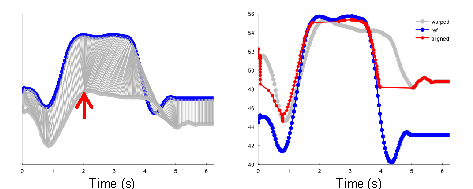
\includegraphics[scale=1.1, draft=false ]{./figures/dtw.pdf} %ok
	\caption{
		Vanilla implementation of dynamic time warping applied to very dissimilar trajectories.
		The plot at the left shows how the time indexes of the reference and warped trajectories relate to each other.
		Note that for a single index in one trajectory, multiple indexes of the other trajectory are allocated due to the minimum distance. One case is indicated by the arrow at time 2 seconds. The consequence of such repetitive correspondence is that the resulting aligned trajectory may present discontinuities (right).
	}
	\label{fig:dtw}
\end{figure}
 
As shown in Fig.~\ref{fig:dtwss}(a) shows the mapping between the time indexes of two trajectories.
At the location indicated by the arrow, the vertical segment indicates the issue of discontinuity, which leads to unnatural alignment.
This issue is usually solved with a slope constraint heuristic.
In this paper we propose solving this issue by forcing a continuous and smooth warping function as shown in Fig.~\ref{fig:dtwss}(b).
This approach generates a one-to-one association of the time indexes which is naturally fit for local optimization of the function $f(\bi \theta)$.

\begin{figure} 
	\centering
	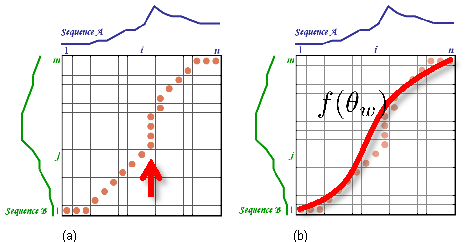
\includegraphics[scale=1.1, draft=false ]{./figures/dtwss.pdf} %ok
	\caption{
	(a) Index mapping with DTW \cite{dtw_webpage}. The part indicated by the arrow causes discontinuities in the trajectory, which is unnatural for physical dynamical systems.
	(b) We propose solving the slope problem by using a warping function that is continuous and smooth by construction. The algorithm forces a one-to-one association of indexes which is more suitable for dynamical systems.
	}
	\label{fig:dtwss}
\end{figure}

